\chapter{Selecci\'on de contenido de expresiones referenciales}
\label{sec:seleccion}

La selecci\'on de cuales propiedades y/o relaciones con otros objetos incluir en una expresi\'on referencial depender\'a del prop\'osito que tengamos para dicha expresi\'on referencial, claramente ser\'a muy distinta la expresi\'on si nuestro objetivo es dar la m\'inima expresi\'on referencial que identifique al objeto que si nuestro objetivo es ser colaborativos con nuestro interlocutor, el la vida hay muchas cosas que nos ayudan a darnos cuenta si nuestro interlocutor identific\'o el objeto target, como ser la expresi\'on de sorpresa nos daria una pauta de que no esta entendiendo lo que le queremos decir, pero cuando queremos hacer esa generaci\'on autom\'atica normalmente ya no poseemos esa clase de informaci\'on.

En esta tesis nos vamos a enfocar la selecci\'on de contenidos de las expresiones referenciales como la gente har\'ia, para ello vamos a usar corpus de expresiones referenciales para aprender como realizan esta tarea los humanos.

En este cap\'itulo daremos una introducci\'on a la generaci\'on autom\'atica de expresiones referenciales y explicaremos los algoritmos m\'as conocidos en el \'area.


\textcolor{blue}{me parece que aca podrian ir estas 2 secciones o fusionarlas en una, me gustaria poner un ejmeplo, no se si aca o en el 1}

\section{Propiedades de las ER}

\section{Propiedades de los Algoritmos GER}


\section{Generaci\'on autom\'atica de expresiones referenciales}

El desaf\'io de la generaci\'on autom\'atica de contenido para las expresiones referenciales viene dado porque una computadora no sabe cuales son las propiedades m\'as sobresalientes de un objetos

\section{Algoritmos de REG}

Cada objeto o entidad tiene un tipo, ciertas propiedades o caracter\'isticas y los valores de esas propiedades, que incluso pueden ser relaciones con otros objetos. 

Por ejemplo: Que cosa es?(el tipo) Una pelota. Tiene color? Si. Que color? Rojo. Esta al lado de otro objeto? Si. Cual? El cubo azul.

Con estos datos tenemos una base de conocimento (en ingles knowlege base KB), estos datos se pueden organizar en jerarquias, por ejemplo: conjunto de animales, conjunto de mamiferos, conjunto de insectos. Algunos conjuntos pueden estar contenidos en otros, es decir algunos objetos o entidades pueden compartir caracter\'isticas.

Si tenemos 100 caracter\'isticas de una persona, y con esas caracter\'isticas se pudiera identificar un\'ivocamente a una persona, un sistema que diera que las 100 caracter\'isticas no ser\'ia un sistema que suene muy natural, ya que una persona no dar\'ia 100 propiedades para identicar a una persona particular. As\'i podr\'iamos decir que las expresiones referenciales variaran segun la cantidad de informaci\'on uqe den, si dan la m\'inima informaci\'on para identificarlas un\'ivocamente seran minimales, si dan m\'as informaci\'on estaran sobreespecificadas, pero en el caso de dar m\'as de la m\'inima informaci\'on... cu\'anta m\'as dar?

El sistema deber\'ia tener una lista del orden de preferencia de los atributos a usar. 

Para una persona identificar ciertos atributos puede ser m\'as f\'acil que identificar ciertos otros, por ejemplo cierto color verde podria ser m\'as complicado de identificar que el tama\~no. Notar que cuando decimos el tama\~no podemos decir ``grande'' y tenemos como marco de referencia a los objetos de la escena, en ese contexto un objeto es ``grande''.

Para un algoritmo entonces, ser\'ian cuestiones importantes de tener en cuenta: 

\begin{itemize}
 \item Que propiedades o relaciones incluir
 \item Cuando terminar (dar la expresi\'on minimal? o dar una expresi\'on sobreespecificada, si es sobreespecifica, que tan sobreespecificada?)
 \item Que orden de preferencias seguir
 \item Hacer o no backtraking
 \item Incluir o no negaciones
\end{itemize}



%\subsection{GREEDY}

%Este algoritmo de Dale~\cite{dale89} busca sobre todo el conjunto de propiedades del target y elije el subconjunto m\'as chico posible que identifica un\'{i}vocamente al objeto target entre los distractores en la escena considerada como se muestra en el siguiente algoritmo.\\

%\begin{figure}[ht]
%\begin{center}
%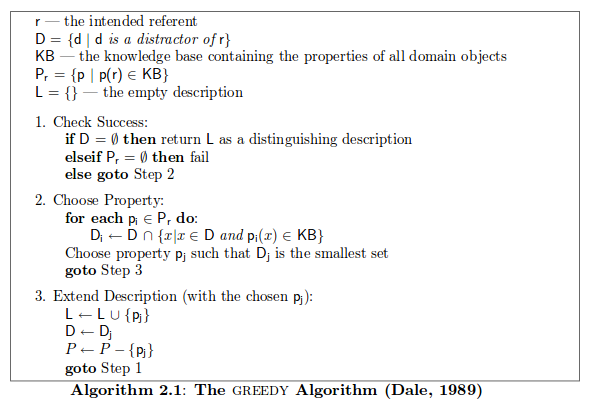
\includegraphics[width=8.5cm]{figures/greedy.png}\\[0pt]
%\caption{Interface del experimento}
%\label{fig-greedy}
%\end{center}
%\end{figure}

%r - el objeto target\\
%D = \{d|d es un distractor de r\}\\
%KB - la base de conocimiento que contiene las propiedades de todos los objetos\\
%$P_{r}$ = $\{p|p(r) \in KB\}$\\
%L = $\{\}$ - la descripci\'on vac\'{i}a\\
%\\
%1. Chequea \'exito:\\
%    \textbf{if} D = $\emptyset$ \textbf{then} return L como una ER que distingue al target r
%    \textbf{elseif} $P_{r}$ = $\emptyset$ \textbf{then} fail
%    
%\textbf{else goto} Paso 2 \\
%\\
%2. Elegir Propiedad:
% \textbf{for each} $p_{i}$ $\in$ $P_{r}$ \textbf{do}:
%    $D_{i}$ $\leftarrow$ D $ \cap$ \{x|x $\in$ D and $p_{i}$ (x) $\in$ KB\}
%    Elegir la propiedad $p_{j}$ tal que $D_{j}$ es el conjunto m\'as chico (es decir la que elimina m\'as distractores) \textbf{goto} Paso 3\\
%\\    
%3. Agregar $p_{j}$ a la descripci\'on actual\\
%L $\leftarrow$ L $\cup$ \{$p_{j}$\}\\
%D $\leftarrow$ $D_{j}$\\
%P $\leftarrow$ P -\{$p_{j}$\}\\
%\textbf{goto} Paso 1\\



%%Dado un dominio D que contiene un target referente r y un conjunto de distractores, una base de conocimiento KB que contiene las propiedades de los objetos.
%%Un conjunto de propiedades verdaderas para r, y una descripcion L inicialmente vac\'{i}a.

%Este algoritmo es de orden NP-complete

\subsection{Incremental}

Se describe a continuaci\'on el algoritmo Incremental de Dale \& Reiter el cual reduce la complejidad del algoritmo Greedy cambiando que en vez de chequear cual propiedad es la que elimina m\'as distractores, eligiendo la que sigue en la lista de propiedades ordenada seg\'un preferencia y que elimina al menos un distractor. Este algoritmo es de orden polinomial.\\


\fbox{ \begin{minipage}{150mm}

r - el objeto target que queremos identificar\\
D = \{d|d es un distractor de r\}\\
KB - la base de conocimiento que contiene las propiedades de todos los objetos\\
$P_{r}$ = $\{p|p(r) \in KB\}$ ordenado seg\'un preferencia de propiedades\\
L = $\{\}$ - la descripci\'on vac\'{i}a\\

1. Chequea \'exito:\\
    \textbf{if} D = $\emptyset$ \textbf{then} return L como una ER que distingue al target r
    \textbf{elseif} $P_{r}$ = $\emptyset$ \textbf{then} fail\\
\textbf{else goto} Paso 2 \\
\\
2. Seleccionar Propiedad:\\
 \textbf{for each} $p_{i}$ $\in$ $P_{r}$ \textbf{do}:\\
 \textbf{if} \{x|x $\in$ $D_{i}$ and $p_{i}$ (x) $\in$ KB\} $\neq$ $\emptyset$\\
 \textbf{then} elegir $p_{j}$ (el la primer propiedad en el orden que elimima al menos un distractor) e \textbf{goto} Paso 3\\
 \textbf{else} $P_{r}$ =$P_{r}$ -$p_{j}$\\
 \textbf{goto} Paso 1\\
      \\    
3. Agregar $p_{j}$ a la descripci\'on actual\\
L $\leftarrow$ L $\cup$ \{$p_{j}$\}\\
D $\leftarrow$ $D_{j}$\\
P $\leftarrow$ P -\{$p_{j}$\}\\
\textbf{goto} Paso 1\\
\end{minipage}}
%\begin{figure}[ht]
%\begin{center}
%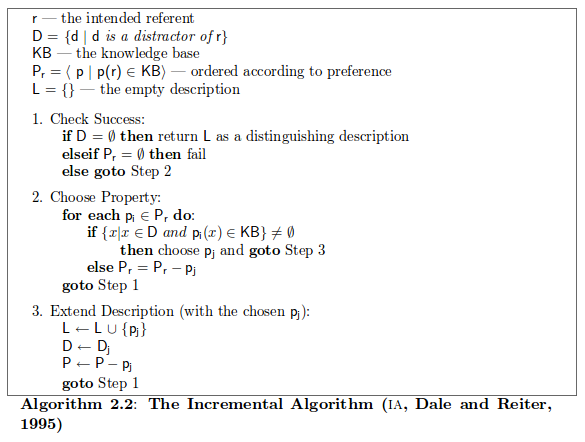
\includegraphics[width=8.5cm]{figures/incremental.png}\\[0pt]
%%\caption{Interface del experimento}
%\label{fig-incremental}
%\end{center}
%\end{figure}

\subsection{Graph}

El dominio que incluye al target y los distractores es representado como un grafo dirigido etiquetado. La representaci\'on gr\'afica de una escena visual se modela cada objeto de la escena como un v\'ertice en el grafo. Los atributos at\'omicos como color, tipo o tama\~no
se representan como un loop en el correspondiente nodo. Ellos est\'an etiquetados con los nombres de atributos y los valores que el objeto en cuesti\'on tiene para estas propiedades. Las relaciones entre objetos, por ejemplo abajo, arriba se modelan como aristas entre los v\'ertices correspondientes.

Para generar una descripci\'on distintiva, el algoritmo de b\'usqueda basado en el gr\'afo
busca un subgrafo del grafo que identifica al target un\'{i}vocamente.

Comenzando con el subgrafo que contiene un solo v\'ertice, que representa al target, se realiza una b\'usqueda en primer lugar a lo ancho sobre el arbol conectado al subgrafo encontrado hasta ahora. Se busca en el espacio de manera exhaustiva,
pero utiliza una heur\'{i}stica basada en el costo (descripto a continuaci\'on) que es capaz de podar el espacio de b\'usqueda.

Informalmente, un subgrafo refiere al target si y s\'olo si puede ser
`Colocado sobre 'el gr\'afico de dominio de tal manera que el v\'ertice que representa subgrafo
el objeto de destino se puede `coloca sobre 'el v\'ertice del objetivo en el gr\'afico de dominio,
y cada uno de los bordes marcados en el subgrafo puede ser `coloca sobre 'un correspondiente
borde en el gr\'afico de dominio con la misma etiqueta y el mismo sentido. Por otra parte,
un subgrafo es distinguir si y s\'olo si se puede `coloca sobre 'exactamente un
v\'ertice en el gr\'afico de dominio. La noci\'on informal de un gr\'afico que se coloca sobre `'
otro corresponde al concepto gr\'afico-te\'orico matem\'atico de
subgrafo isomorfismo, Se modelan como aristas entre los v\'ertices correspondientes.


\subsection{Bisimulaci\'on}


En este cap\'itulo daremos una introducci\'on a l\'ogicas de descripci\'on (DL del acr\'onimo en ingl\'es description logic) y luego daremos el algoritmo en el cual nos basamos en esta tesis.

Hay distintas l\'ogicas, y entre ellas se diferencian por como se generan, vamos a explicar \alc y \el.

\emph{F\'ormulas} (o \emph{concepts}) $\varphi$ de $\alc$ son generadas por la siguiente gram\'atica;
$$
\varphi,\varphi' ::= \top \mid p \mid \neg \varphi \mid \varphi \sqcap \varphi'
\mid \exists R. \varphi
$$
donde $p$ es el conjunto de los s\'imbolos proposicionales \prop y $R$ es el de los s\'imbolos relacionales \rel. $\el$ es la parte sin negaci\'on de $\alc$.

Las f\'ormulas de ambos $\alc$ y $\el$ son interpretadas en modelos relacionales de primer orden $\gM = (\Delta,\interp{\cdot})$ donde
$\Delta$ es un conjunto no vac\'io y $\interp{\cdot}$ es una funci\'on de interpretaci\'on tal que:
$$
\begin{array}{ccl}
\interp{p} & \subseteq & \Delta  \mbox{ for $p \in \prop$}\\
\interp{R} & \subseteq & \Delta \times \Delta  \mbox{ for $R \in \rel$}\\
\interp{\neg \varphi} & = & \Delta - \interp{\varphi}\\
\interp{\varphi \sqcap \varphi'} & = & \interp{\varphi} \cap \interp{\varphi'}\\
\interp{\exists R.\varphi} & = & \{i \mid \mbox{for some } i', (i,i') \in \interp{R}\\
& & \mbox{ and } i' \in \interp{\varphi} \}.\\
\end{array}
$$

\begin{figure}[ht]
\begin{center}
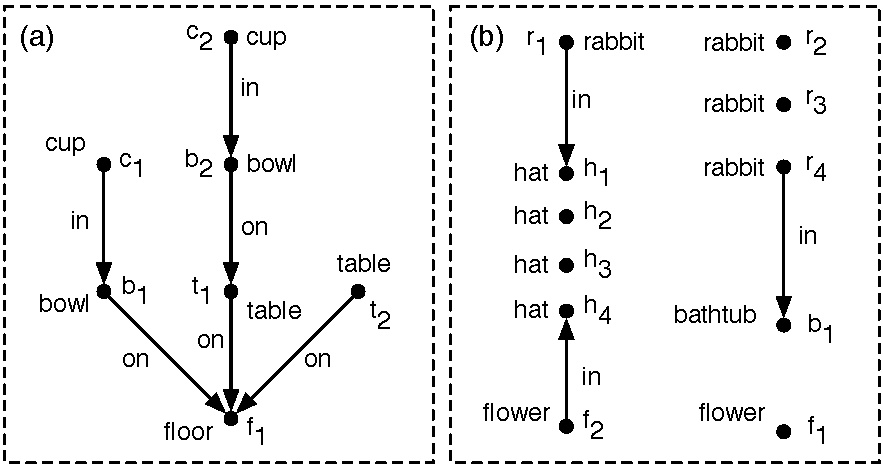
\includegraphics[width=8.5cm]{figures/pic-dale-haddock.pdf}\\[0pt]
\caption{}
\label{fig:dale-haddock}
\end{center}
\end{figure}


Cada f\'ormula de una descripci\'on l\'ogica denota un conjunto de objetos del dominio; por lo tanto podemos usar tales f\'ormulas para describir conjuntos. Por ejemplo en el modelo de la Figura.~\ref{fig:dale-haddock}b, la f\'ormula
$\mathsf{flower}$ denota el conjunto $\{f_1,f_2\}$; La f\'ormula
$\mathsf{flower} \sqcap \exists \mathsf{in}.\mathsf{hat}$ denota
$\{f_2\}$; y la f\'ormula $\mathsf{flower} \sqcap \neg
\exists \mathsf{in}.\mathsf{hat}$ denota $\{f_1\}$.

Diferentes l\'ogicas de descripci\'on difieren en los conectores que permiten: Mientras que \alc\ permite negaci\'on, \el\
no permite. 

Hay muchas otras l\'ogicas de descripci\'on en la literatura por ejemplo 

$\mathcal{CL}$ (\el\ sin el cuantificador existencial, i.e., only
conjunctions of atoms); $\mathcal{PL}$ (\alc\ l\'ogica propocisional); y
$\mathcal{ELU}_{(\neg)}$ (\el\ m\'as disjunci\'on y negaci\'on at\'omica).

Usaremos una noci\'on de preservaci\'on de f\'ormulas que llamaremos
\emph{similarity}. Para cualquier DL $\gL$, diremos que un individual $i$ es \emph{\gL-similar} a $i'$ en un modelo dado $\gM$
si para cualquier f\'ormula $\varphi \in \gL$ tal que $i \in
\interp{\varphi}$, tambi\'en tenemos que $i' \in \interp{\varphi}$.
Equivalentemente, no hay $\gL$-f\'ormula que se mantenga para $i$ pero no para
$i'$.  Diremos que \emph{\gL-conjunto de similaridad } de alg\'un individual
$i$ es el conjunto de todos los individuales a los cuales $i$ es \gL-similar.

Notar que la similaridad no es necesariamente una relaci\'on sim\'etrica: Por ejemplo: $f_1$ es \el-similar a $f_2$ en
Fig.~\ref{fig:dale-haddock}b, pero $f_2$ no es \el-similar a $f_1$
(satisface la f\'ormula $\exists \mathsf{in}.\mathsf{hat}$ y $f_1$
no la satisface).  De todas maneras, \alc-similaridad es una relaci\'on sim\'etrica porque
el languaje contiene negaci\'on; y en consecuencia, $f_1$ no es \alc-similar
a $f_2$ porque este tampoco satisface $\neg \exists
\mathsf{in}.\mathsf{hat}$.  Porque \alc\ es m\'as expresivo que \el,
esto es, para alg\'un indivdual $a$ es posible ser \el-similar pero
no \alc-similar a alg\'un individual $b$, pero no viceversa.


La idea es transformar el problema de GRE al problema de computar una f\'ormula de DL cuya extensi\'on es el elemento target (o los elementos targets) ya que una f\'ormula describe un conjunto.

Las RE que involucran relaciones han recibido m\'as atenci\'on recientemente;
especialmente en el contexto de las expresiones referenciales espaciales en 
generaci\'on (por ejemplo,~\cite{kelleher06:increm}),
donde es particularmente natural utilizar expresiones que implican 
relaciones espaciales, tales como ``la pelota en la parte superior del cubo''. Sin embargo, el
algoritmo cl\'asico
por~\cite{dale91:gener} ha demostrado ser
incapaz de generar RE satisfactorias en la pr\'actica (v\'ease el an\'alisis sobre
el~\emph{cabinet corpus}
en~\cite{viethen06:_algor_for_gener_refer_expres}). Adem\'as, el
Dale y Haddock algoritmo y muchos de sus sucesores (tales
como~\cite{kelleher06:increm}) son vulnerables a
el problema de la \emph{regresi\'on infinita}, donde el algoritmo entra en un
bucle infinito, saltando hacia atr\'as y hacia adelante entre las descripciones para dos
individuos emparentados, como en `` el libro sobre la mesa que soporta una
libro sobre la mesa \ldots ''

%REs involving relations have received increasing attention recently;
%especially in the context of spatial referring expressions in situated
%generation (e.g., \cite{kelleher06:increm}),
%where it is particularly natural to use expressions involving spatial
%relations such as ``the ball on top of the cube.''  However, the
%classical algorithm
%by~\cite{dale91:gener} was shown to be
%unable to generate satisfying REs in practice (see the analysis over
%the \emph{cabinet corpus}
%in~\cite{viethen06:_algor_for_gener_refer_expres}).  Furthermore, the
%Dale and Haddock algorithm and many of its successors (such
%as~\cite{kelleher06:increm}) are vulnerable to
%the problem of \emph{infinite regress}, where the algorithm enters an
%infinite loop, jumping back and forth between descriptions for two
%related individuals, as in ``the book on the table which supports a
%book on the table \ldots''

%\cite{arec2:2008:Areces,arec:usin11} have proposed low complexity
%algorithms for the generation of relational REs
%%(including references to sets) 
%that eliminate the risk of infinite regression.  These algorithms are
%based on variations of the partition refinement algorithms
%of~\cite{paig:thre87}.  The information provided by a given scene
%is interpreted as a relational model whose objects are classified into
%sets that fit the same description.  This classification is
%successively \emph{refined} till the target is the only element
%fitting the description of its class.  The existence of an RE depends
%on the information available in the input scene, and on the expressive
%power of the formal language used to describe elements of the
%different classes in the refinement.


\cite{arec2:2008:Areces,arec:usin11} han propuesto algoritmos de baja complejidad
 para la generaci\'on de ER relacionales
% (incluyendo referencias a juegos)
que eliminan el riesgo de regresi\'on infinita. Estos algoritmos son
basado en variaciones de los algoritmos de refinamiento partici\'on
de~\cite{paig:thre87}. La informaci\'on proporcionada por una escena dada
se interpreta como un modelo relacional cuyos objetos se clasifican en
juegos que se adapten a la misma descripci\'on. Esta clasificaci\'on es
sucesivamente \emph{refinado} hasta el blanco es el \'unico elemento
ajuste de la descripci\'on de su clase. La existencia de un RE depende
en la informaci\'on disponible en la escena de entrada, y en la expresiva
poder del lenguaje formal utilizado para describir los elementos de la
diferentes clases en el refinamiento.

%Refinement
%algorithms %presented in~\cite{arec2:2008:Areces,arec:usin11}
%effectively compute REs for all individuals in the domain, at the same
%time. The algorithms always terminate returning a formula of the
%formal language chosen that uniquely describes the target (if the
%formal language is expressive enough to identify the target in the
%input model).
%\cite{arec2:2008:Areces}
%show that the refinement algorithm using the description language \el  is capable of generating 67\% of 
%the relational REs in the~\cite{viethen06:_algor_for_gener_refer_expres} dataset, when all possible orders of the relations in the domain are considered. This is in sharp contrast with the analysis 
%done in~\cite{viethen06:_algor_for_gener_refer_expres} over the cabinet corpus, of algorithms based in Dale and Reiter's original proposal.    

Los algoritmos de refinamiento
% presenta en ~ \ cite {arec 2: 2008: Areces, arec: usin11}
calcular efectivamente ER para todos los objetos en el dominio, al mismo
tiempo. Los algoritmos siempre terminan devolviendo una f\'ormula del
lenguaje formal elegido que describe un\'{i}vocamente el objetivo (si el
lenguaje formal es suficientemente expresiva para identificar el target en el
modelo de entrada).

%Refinement algorithms for GRE are based on the following basic idea:
%given a scene $S$, the objects appearing in $S$ are successively
%classified according to their properties into finer and finer
%classes. A description (in some formal language $\mathcal{L}$) of each
%class is computed every time a class is refined. The procedure always
%stops when the set of classes stabilizes, i.e., no further refinement
%is possible with the information available in the scene\footnote{Of
%  course, if we are only interested in a referring expression for a
%  given target we can stop the procedure as soon as the target is the
%  only element of some of the classes.}.  If the target element is in
%a singleton class, then the formal description of that class is a
%referring expression; otherwise the target cannot be unequivocally
%described (in 

Algoritmos de refinamiento para GRE se basan en la siguiente idea b\'asica:
dada una escena $S$, los objetos que aparecen en $S$ son sucesivamente
clasificados de acuerdo con sus propiedades en m\'as y m\'as fino
clases. Una descripci\'on (en alg\'un lenguaje formal de $\mathcal{L}$) de cada
clase se calcula cada vez que una clase es refinado. El procedimiento siempre
se detiene cuando el conjunto de clases se estabiliza, es decir, no mayor refinamiento
que es posible con la informaci\'on disponible en la escena \footnote{De
   Por supuesto, si s\'olo estamos interesados en una expresi\'on que se refiere a un
   objetivo dado que puede detener el procedimiento en cuanto el objetivo es la
   \'unico elemento de algunas de las clases.}. Si el elemento de destino est\'a en
una clase singleton, entonces la descripci\'on formal de esa clase es un
refiri\'endose expresi\'on; de lo contrario el destino no puede ser inequ\'{i}vocamente
descrito (en $\mathcal{L}$).

%It is clear that a scene can be encoded in different ways as a
%relational model (for example in \ref{figure22}, we could argue that
%$e_1$ is also \emph{leftof} $e_2$, not considered because they are no
%touching). The algorithm assumes that these issues have been resolved
%and that the model encodes a suitable representation of the scene we
%want to describe.  Moreover, we will assume that all relations are
%\emph{binary}.  We will not consider relations of arity greater than
%two (relations of higher arity can be encoded as binary relations via
%reification, if necessary).

Est\'a claro que una escena puede ser codificado en diferentes formas como una
modelo relacional (por ejemplo, en \ref{figure22}, podr\'{i}amos argumentar que
$e_1$ es tambi\'en \emph{leftof} $e_2$, no se considera porque hay
tocando). El algoritmo asume que estas cuestiones se han resuelto
y que el modelo codifica una representaci\'on adecuada de la escena que
querer describir. Por otra parte, vamos a suponer que todas las relaciones son
\emph{binario}. No vamos a considerar las relaciones de aridad mayor que
dos (relaciones de mayor aridad pueden codificarse como relaciones binarias v\'{i}a
reificaci\'on, si es necesario).

%On termination, the algorithm computes what are called the
%$\mathcal{L}$-similarity classes of the input model $\gM$.
%Intuitively, the referring expression ``\textsf{ball}'' and ``\textsf{cube}''  are more specific and then contain more information than $\top$.


Tras la resoluci\'on, el algoritmo calcula lo que se llama la
$\mathcal{L}$ - clases de semejanza del modelo de entrada de $\gM$.

%There is many $\mathcal{L}$, we will name $\alc$ and $\el$

%ACA VOY A PONER gramatica para generar... ALC y EL no quedaria bien aca, hay que ver lo agregamos antes o no hace falta
In what follows, we use formulas of the $\el$ description logic
language~\cite{baad:desc03} to describe refinement classes
\footnote{Notice, though, that the particular formal language used is
  independent of the main algorithm, and different
  add$_{\mathcal{L}}$($\varphi$,\RE) functions can be used depending
  on the language involved.}.  As discussed
in~\cite{arec2:2008:Areces}, this language is suitable for describing
conjunctive and relational REs, which are the ones we find in corpora.

 The input to the algorithm will be a relational model $\mathcal{M} =
 \tup{\Delta, \interp{\cdot}}$, where $\Delta$ is the non-empty domain
 of objects in the scene, and $\interp{\cdot}$ is an interpretation
 function that assigns to all properties in the scene their intended
 extension.  For example, the scene shown in Figure~\ref{figure22}
 could be represented by the model $\gM=\tup{\Delta,\interp{\cdot}}$
 shown in Figure~\ref{GRE3D7-stimulus-graph}; where $\Delta =
 \{e_1,\ldots,e_7\}$, and $\interp{\textsf{red}}$ is $\{e_2, e_4, e_5,
 e_7\}$.

$\top$ is a formula that represents the most general description whose
interpretation includes all elements of the model. It could be realize
as the RE with the noun ``\textsf{thing}''. We say that a formula is
\emph{subsumed} by other formulas, if it extension can be cover by the
union of the extensions of the other formulas. For example, in
Figure~\ref{figure22}, $\top$ is subsumed by ``\textsf{ball}'' and
``\textsf{cube}'', because $\interp{\top}$ = $\interp{\textsf{ball}}
\cup \interp{\textsf{cube}}$.
%= $\{e_2, e_4, e_6, e_7\}$, it is $\{e_1, e_2, e_3, e_4, e_5, e_6, e_7\}$ = $\{e_1, e_3, e_5\} \cup \{e_2, e_4, e_6, e_7\}$. 
Intuitively the formula ``\textsf{cube}'' or ``\textsf{ball}'' have more information than $\top$, for each element of $\top$, there is a formula that gives more information, say ``\textsf{cube}'' is more informative than say ``\textsf{thing}''.\\

In the following we will explain an example of execusion of the
algorithm shown in Figure~\ref{algoritmoOriginal} taking into account
the $\el$ logic language. This algorithm where first presented
in~\cite{arec2:2008:Areces}.

\begin{figure}[h!]
\begin{center}
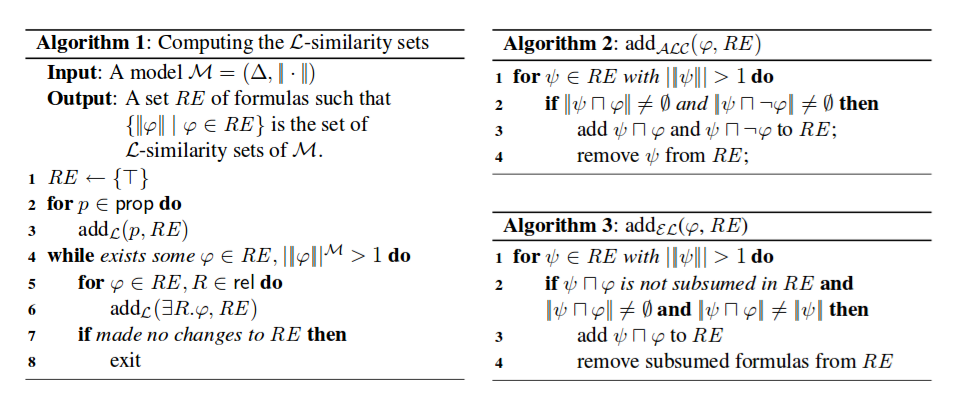
\includegraphics[width=\textwidth]{images/algoritmoOriginal.png}
\end{center}
\vspace*{-2em}
\caption{Algorithms for GRE with Description Logic}
\label{algoritmoOriginal}
\end{figure}

\subsection{An example of execution}

We will run the algorithm for the Scene~\ref{figure22}, the algorithm
start with a fixed list of properties and relations, suppose that
those lists are the following:

ordered properties (prop): \textsf{ball}, \textsf{cube}, \textsf{red}, \textsf{yellow}, \textsf{small}, \textsf{large}.\\
ordered relations (rel): \textsf{leftof}, \textsf{rightof}, \textsf{ontopof}, \textsf{bellowof}.

\begin{figure}
\begin{center}	
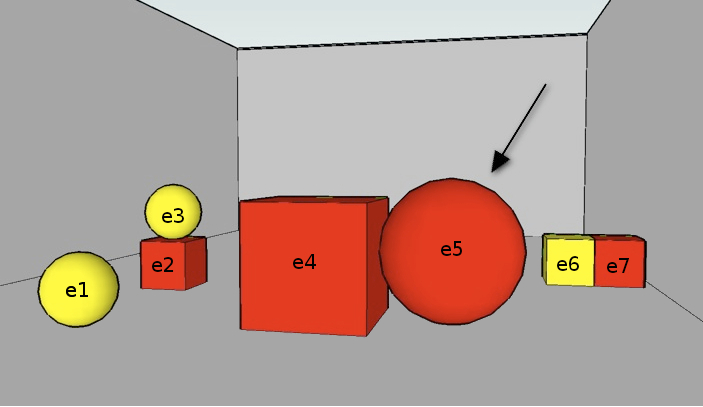
\includegraphics[width=.5\textwidth]{images/22.jpg}
\end{center}
\vspace*{-1.5em}
\caption{A 3D scene of geometric figures}\label{figure22}
\end{figure}

\begin{figure}
\begin{minipage}[b]{0.6\linewidth}
\centering
\begin{tikzpicture}
  [
    n/.style={circle,fill,draw,inner sep=3pt,node distance=1.4cm},
    aArrow/.style={->, >=stealth, semithick, shorten <= 2pt, shorten >= 2pt},
  ]
 \node[n,label=above:$e_1$,label=below:{
    \relsize{-1}$\begin{array}{c}
      \nLeft\\[-2pt]
      \nSmall\\[-2pt] 
      \nYellow \\[-2pt] 
      \nBall\end{array}$}] (a) {};

 \node[n,label=above:$e_2$,label=below:{
    \relsize{-1}$\begin{array}{c}
      \nLeft\\[-2pt]
      \nSmall\\[-2pt] 
      \nRed\\[-2pt] 
      \nCube\end{array}$}, right of=a] (b) {};

 \node[n,label=below:$e_3$,label=above:{
    \relsize{-1}$\begin{array}{c}
      \nTop\\[-2pt]
      \nLeft\\[-2pt]
      \nSmall\\[-2pt] 
      \nYellow\\[-2pt] 
      \nBall\end{array}$}, above of=b] (c) {};

 \node[n,label=above:$e_4$,label=below:{
    \relsize{-1}$\begin{array}{c}
      \nBig\\[-2pt] 
      \nRed\\[-2pt] 
      \nCube\end{array}$}, right of=b] (d) {};

 \node[n,label=above:$e_5$,label=below:{
    \relsize{-1}$\begin{array}{c}
      \nBig\\[-2pt] 
      \nRed\\[-2pt] 
      \nBall\end{array}$}, right of=d] (e) {};

 \node[n,label=above:$e_6$,label=below:{
    \relsize{-1}$\begin{array}{c}
      \nSmall\\[-2pt] 
      \nYellow\\[-2pt] 
      \nCube\end{array}$}, right of=e] (f) {};

 \node[n,label=above:$e_7$,label=below:{
    \relsize{-1}$\begin{array}{c}
      \nSmall\\[-2pt] 
      \nRed\\[-2pt] 
      \nCube\end{array}$}, right of=f] (g) {};

 \draw [aArrow,bend right=90] (b) to node[auto,swap]{\relsize{-1}$\nBelow$} (c);
 \draw [aArrow,bend right=90] (c) to node[auto,swap]{\relsize{-1}$\nOntop$} (b);

 \draw [aArrow,bend right=30] (d) to node[auto,swap]{\relsize{-1}$\nLeftof$} (e);
 \draw [aArrow,bend right=30] (e) to node[auto,swap]{\relsize{-1}$\nRightof$} (d);

 \draw [aArrow,bend right=30] (f) to node[auto,swap]{\relsize{-1}$\nLeftof$} (g);
 \draw [aArrow,bend right=30] (g) to node[auto,swap]{\relsize{-1}$\nRightof$} (f);

 \draw[dotted] (-.4,-1.7) rectangle (7.5,3.3);

 \end{tikzpicture}
\caption{Scene as a relational model}\label{GRE3D7-stimulus-graph}
\end{minipage}
\end{figure}


The algorithm always ends, and return RE, a set of formulas that describes each element in the domain (if that formula exists).\\

In the begining RE=$\{\top\}$ and its $\interp{\top}$ = $\{e_1, e_2, e_3, e_4, e_5, e_6, e_7\}$\\

The first loop for of the algorithm is in the properties. For each property realize add$_\el$ ($\varphi$, RE),

A formula $\varphi$ will be added to RE if its interpretation has at least one element, then for each formula $\psi$ in RE the conjunction 
$\varphi  \wedge \psi$ need to be not subsumed in RE, the $\interp{\varphi \cup \psi}$ need to be not empty, and its interpretation need to be distinct of $\interp{\psi}$. Then the subsumed formulas will be clean.

The first property is \textsf{ball}, RE = \{$\top$, \textsf{ball}\}, then the following property is \textsf{cube}, RE = \{$\top$, \textsf{ball}, \textsf{cube}\}, but now the $\interp{\textsf{ball}}$ = $\{e_1, e_3, e_5\}$, $\interp{\textsf{cube}}$ = $\{e_2, e_4, e_6, e_7\}$, so, we can delete $\top$, because it is subsumed to the two other formulas. The turn is now for the property \textsf{red}, $\interp{\textsf{red}}$ is: $\{e_2, e_4, e_5, e_7\}$, doing the intersection with the $\interp{.}$ of each formula in RE we obtain, $\{e_5\}$ and $\{e_2, e_4, e_7\}$, RE = $\{\textsf{ball}, \textsf{cube}, \textsf{ball} \wedge \textsf{red}, \textsf{cube} \wedge \textsf{red}\}$, following with \textsf{yellow}, we have, $\interp{\textsf{yellow}}$ = $\{e_1, e_3, e_6\}$ and we obtain RE = $\{\textsf{ball} \wedge \textsf{yellow}, \textsf{cube} \wedge \textsf{yellow}, \textsf{ball} \wedge \textsf{red}, \textsf{cube} \wedge \textsf{red}\}$. Note than here we already delete the formula \textsf{ball} because it was subsumed, and the formula \textsf{cube} too.
Doing the same with \textsf{small} we have RE = $\{\textsf{ball} \wedge \textsf{yellow} \wedge \textsf{small}, \textsf{cube} \wedge \textsf{yellow} \wedge \textsf{small}, \textsf{ball} \wedge \textsf{red}, \textsf{cube} \wedge \textsf{red}, \textsf{cube} \wedge \textsf{red} \wedge \textsf{small}\}$. Next property is \textsf{large} so, we have RE = $\{\textsf{ball} \wedge \textsf{yellow} \wedge \textsf{small}, \textsf{cube} \wedge \textsf{yellow} \wedge \textsf{small}, \textsf{ball} \wedge \textsf{red}, \textsf{cube} \wedge \textsf{red} \wedge \textsf{large}, \textsf{cube} \wedge \textsf{red} \wedge \textsf{small}\}$. Note that here we cannot add \textsf{large} to a formula $\textsf{red} \wedge \textsf{cube}$ because its interpretation has only one element, and the condition say that it need to have more than one.

Until now RE = $\{\textsf{ball} \wedge \textsf{yellow} \wedge \textsf{small}, \textsf{cube} \wedge \textsf{yellow} \wedge \textsf{small}, \textsf{ball} \wedge \textsf{red}, \textsf{cube} \wedge \textsf{red} \wedge \textsf{large}, \textsf{cube} \wedge \textsf{red} \wedge \textsf{small}\}$ and we have the following extensions: $\{e_1, e_3\}, \{e_6\}, \{e_5\}, \{e_4\}, \{e_2, e_7\}$ respectively. There is two formulas that can be refined more, the  $\textsf{ball} \wedge \textsf{yellow} \wedge \textsf{small}$ and $\textsf{cube} \wedge \textsf{red} \wedge \textsf{small}$ because they have more than one element each, so we enter en in the while cicle of Algorithm 1, in line 4. Now is the turn of relations, the first one is \textsf{leftof}, for each formula $\varphi$ in RE will try to add$_\el$ ($\exists \textsf{leftof}.\varphi$, RE). Note that $\psi$ only can be $\textsf{ball} \wedge \textsf{yellow} \wedge \textsf{small}$ or $\textsf{cube} \wedge \textsf{red} \wedge \textsf{small}$ because those are the ones that its interpretation have more than one element. There is not $\varphi$ and $\psi$ that can be apply. Continuing with \textsf{rightof} we add $\textsf{cube} \wedge \textsf{yellow} \wedge \textsf{small} \wedge \exists \textsf{rightof}. \textsf{cube} \wedge \textsf{red} \wedge \textsf{small}$, and so on with \textsf{topof} we add $\textsf{small} \wedge \textsf{red} \wedge \textsf{cube} \wedge \exists \textsf{ontop}. \textsf{small} \wedge \textsf{yellow} \wedge \textsf{ball}$ and the algorithm ends with RE = $\{\textsf{ball} \wedge \textsf{yellow} \wedge \textsf{small}, \textsf{cube} \wedge \textsf{yellow} \wedge \textsf{small}, \textsf{ball} \wedge \textsf{red}, \textsf{cube} \wedge \textsf{red} \wedge \textsf{large}, \textsf{cube} \wedge \textsf{red} \wedge \textsf{small}, \textsf{cube} \wedge \textsf{yellow} \wedge \textsf{small} \wedge \exists \textsf{rightof}. \textsf{cube} \wedge \textsf{red} \wedge \textsf{small}, \textsf{small} \wedge \textsf{red} \wedge \textsf{cube} \wedge \exists \textsf{ontop}. \textsf{small} \wedge \textsf{yellow} \wedge \textsf{ball}\}$, here all elements are in a singleton class and not further refinement can be done.


%can be applied to $cube \wedge red \wedge small$ but there is no formula which interpretation has more than one element to be apply with this one. The same happen for the other relations, so the algorithm ends.
%its interpretation is $\{e_7\}$ with $\psi$ is $cube \wedge yellow \wedge small$, the others combinations can't be apply because they don't do true the preconditions. The following relation is rightof, 

%leftof, rightof, ontopof, bellowof

%At this point we already have the target in a singleton set. So the formula for it is ``red and ball'', and also for s6 which formula is ``yellow cube''.\\
%As we show this algorithm depends of the order of properties and relations.\\




\section{Aproximaciones emp\'iricas a la soluci\'on de REG}



\subsection{Corpus existente}

\textcolor{blue}{Aca probablemente describa los corpus TUNA y GRE3D7}
\label{sec:corpusGRE}
\label{sec:corpusTUNA}

\subsection{Jette y otros trabajos emp\'iricos}

%http://link.springer.com/chapter/10.1007/978-3-642-15573-4_9
\subsection{M\'etricas de evaluaci\'on/comparaci\'on con corpus}



